\begin{indentitemize}
    \item text
\end{indentitemize}
\begin{figure}[htbp]
\begin{subfigure}{0.48\textwidth}
    \begin{tikzpicture}
    [x=0.1\textwidth, y=0.1\textwidth]
    \draw (0,0) rectangle (10,5);
    \draw[thick] (0.5,4.5) circle(0.3) node{1};
    \filldraw[orange]
        (1,2.2) .. controls (0.8,2.5) ..
        (1.2,3.5) .. controls (1.6,2.5) ..
        (1.4,2.2);
    \filldraw[red]
        (1.2,3) .. controls (1.4,2.5) ..
        (1.2,2.3) .. controls (1,2.5) ..
        (1.2,3);
    \draw[fill=darkgrey]
        (0.2,0.2)--
        (2.2,0.2)--
        (1.4,1.2)--
        (1.4,2.2)--
        (1,2.2)--
        (1,1.2)--
        (0.2,0.2);
    \draw[fill=brightgrey]
        (1.2,3.5)--
        (0.4,3.2)--
        (0.38,3.25)--
        (1.2,3.6)--
        (1.6,3.63)--
        (1.8,3.7)--
        (5,3.7)--
        (5,3.4)--
        (1.8,3.4)--
        (1.6,3.47)--
        (1.2,3.5);
    \filldraw[red,scale=0.5,shift={(11.5,7)}]
        (0,.5)--
        (2,.5)--
        (2,1)--
        (3,0)--
        (2,-1)--
        (2,-.5)--
        (0,-.5);
%    \draw[fill=red]
%        (4,1)--
%        (6,1)--
%        (6,0.5)--
%        (7,1.5)--
%        (6,2.5)--
%        (6,2)--
%        (4,2)--
%        (4,1);
    \draw[fill=brightgrey,shift={(8.5,4.5)}]
        (0,0)--
        (0.025,0.05)--
        (0.525,-0.2)..controls(0.6,-0.25)..
        (0.525,-0.3)--
        (-0.175,-0.65)--
        (-0.16,-1)--
        (-0.11,-1.1)--
        (-0.11,-4)--
        (-0.365,-4)--
        (-0.365,-1.1)--
        (-0.315,-1)--
        (-0.3,-0.65)..controls(-0.25,-0.6)..
        (-0.2,-0.57)--
        (0.48,-0.25)--
        (0,0);
    \end{tikzpicture}
    \subcaption{Forming the pipette}
\end{subfigure}
\hfill
\begin{subfigure}{0.48\textwidth}
    \begin{tikzpicture}
    [x=0.1\textwidth, y=0.1\textwidth]
    \draw (0,0) rectangle (10,5);
    \draw[thick] (0.5,4.5) circle(0.3) node{2};
    \filldraw[water] (0.5,0.5) rectangle (9.5,2.2);
    \draw[fill=grey]
        (0.2,2.5)--
        (0.5,2.5)--
        (0.5,0.5)--
        (9.5,0.5)--
        (9.5,2.5)--
        (9.8,2.5)--
        (9.8,0.2)--
        (0.2,0.2)--
        (0.2,2.5);
    \draw[fill=solution,shift={(5,1.5)},rotate=250,scale=1.2]
        (0,0)--
        (0.025,0.05)--
        (0.525,-0.2)..controls(0.6,-0.25)..
        (0.525,-0.3)--
        (-0.175,-0.65)--
        (-0.16,-1)--
        (-0.11,-1.1)--
        (-0.11,-4)--
        (-0.365,-4)--
        (-0.365,-1.1)--
        (-0.315,-1)--
        (-0.3,-0.65)..controls(-0.25,-0.6)..
        (-0.2,-0.57)--
        (0.48,-0.25)--
        (0,0);
    \draw[fill=brightgrey,shift={(5,1.5)},rotate=250,scale=1.2]
        (-0.11,-4)--
        (-0.11,-2)--
        (-0.365,-1.3)--
        (-0.365,-4)--
        (-0.11,-4);
    \draw[line width=0.006\textwidth,dotted,color=solution]
        (5.02,1.5) to[thick] (5.02,2.2);
    \foreach \i in {0.55,0.66,...,2.55}
        \filldraw[sphere] (\i,2.25) circle (0.05);
    \foreach \i in {7.45,7.56,...,9.45}
        \filldraw[sphere] (\i,2.25) circle (0.05);
    \draw[sphere,->,line width=0.007\textwidth]
        (5.2,1.5)..controls(5.2,2.2)and(5.35,2.25)..
        (7,2.25);
    \end{tikzpicture}
    \subcaption{petri dish}
\end{subfigure}

\begin{subfigure}{0.48\textwidth}
    \begin{tikzpicture}
    [x=0.1\textwidth, y=0.1\textwidth]
    \draw (0,0) rectangle (10,5);
    \draw[thick] (0.5,4.5) circle(0.3) node{3};
    \filldraw[water] (0.5,0.5) rectangle (9.5,1.44);
    \draw[fill=grey]
        (0.2,2.5)--
        (0.5,2.5)--
        (0.5,0.5)--
        (9.5,0.5)--
        (9.5,2.5)--
        (9.8,2.5)--
        (9.8,0.2)--
        (0.2,0.2)--
        (0.2,2.5);
    \foreach \i in {2.25,2.14,...,1.49}
        \filldraw[sphere] (0.55,\i) circle (0.05);
    \foreach \i in {0.55,0.66,...,5.55}
        \filldraw[sphere] (\i,1.49) circle (0.05);
    \draw[fill=substrate]
        (1,0.5) rectangle (2,.7)
        (3,0.5) rectangle (4,.7);
    \draw[sphere,->,ultra thick]
        (1.5,1.3) -- (1.5,0.8);
    \draw[sphere,->,ultra thick]
        (3.5,1.3) -- (3.5,0.8);
    \draw[ultra thick,fill=water]
        (8,1)..controls(8.5,3.8)..
        (10,4.5)--
        (10,4)..controls(9,3.5)..
        (8.5,1);
    \draw[ultra thick,->]
        (8.35,1.4)--(8.5,2.12);
    \end{tikzpicture}
    \subcaption{petri dish}
\end{subfigure}
\hfill
\begin{subfigure}{0.48\textwidth}
    \begin{tikzpicture}
    [x=0.1\textwidth, y=0.1\textwidth]
    \draw (0,0) rectangle (10,5);
    \draw[thick] (0.5,4.5) circle(0.3) node{4};
    \draw[fill=substrate]
        (0.5,0.5) rectangle (2.5,0.7)
        (0.5,1.5) rectangle (2.5,3.5);
    \foreach \i in {1.63,1.9764,...,3.41}
        \foreach \j in {0.6,0.8,...,2.41}
            \filldraw[sphere] (\j,\i) circle (0.095);
    \foreach \i in {1.8032,2.1496,...,3.41}
        \foreach \j in {0.7,0.9,...,2.41}
            \filldraw[sphere] (\j,\i) circle (0.095);
    \foreach \i in {0.6,0.8,...,2.41}
        \filldraw[sphere] (\i,0.795) circle (0.095);
    \coordinate (s) at (7,0);
    \draw[fill=substrate,shift={(s)}]
        (0.5,0.5) rectangle (2.5,0.7)
        (0.5,1.5) rectangle (2.5,3.5);
    \foreach \i in {1.63,1.9764,...,3.41}
        \foreach \j in {0.6,0.8,...,2.41}
            \filldraw[sphere,shift={(s)}] (\j,\i) circle (0.105);
    \foreach \i in {1.8032,2.1496,...,3.41}
        \foreach \j in {0.7,0.9,...,2.41}
            \filldraw[sphere,shift={(s)}] (\j,\i) circle (0.105);
    \foreach \i in {0.6,0.8,...,2.41}
        \filldraw[sphere,shift={(s)}]
            (\i,0.79) ellipse [x radius=0.105,y radius=0.09];
    \filldraw[red,scale=0.5,shift={(9,5)}]
        (0,.5)--
        (2,.5)--
        (2,1)--
        (3,0)--
        (2,-1)--
        (2,-.5)--
        (0,-.5);
    \end{tikzpicture}
    \subcaption{annealing}
\end{subfigure}
\end{figure}

\begin{figure}[htbp]
\begin{subfigure}{0.48\textwidth}
    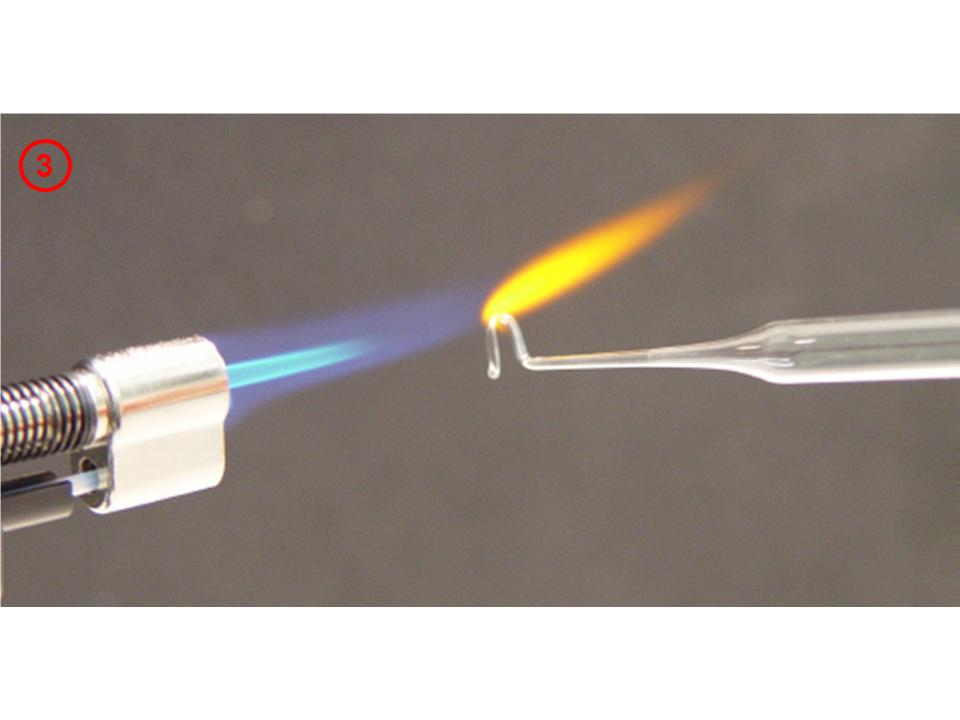
\includegraphics[width=\textwidth]{pipette.jpg}
\end{subfigure}
\hfill
\begin{subfigure}{0.48\textwidth}
    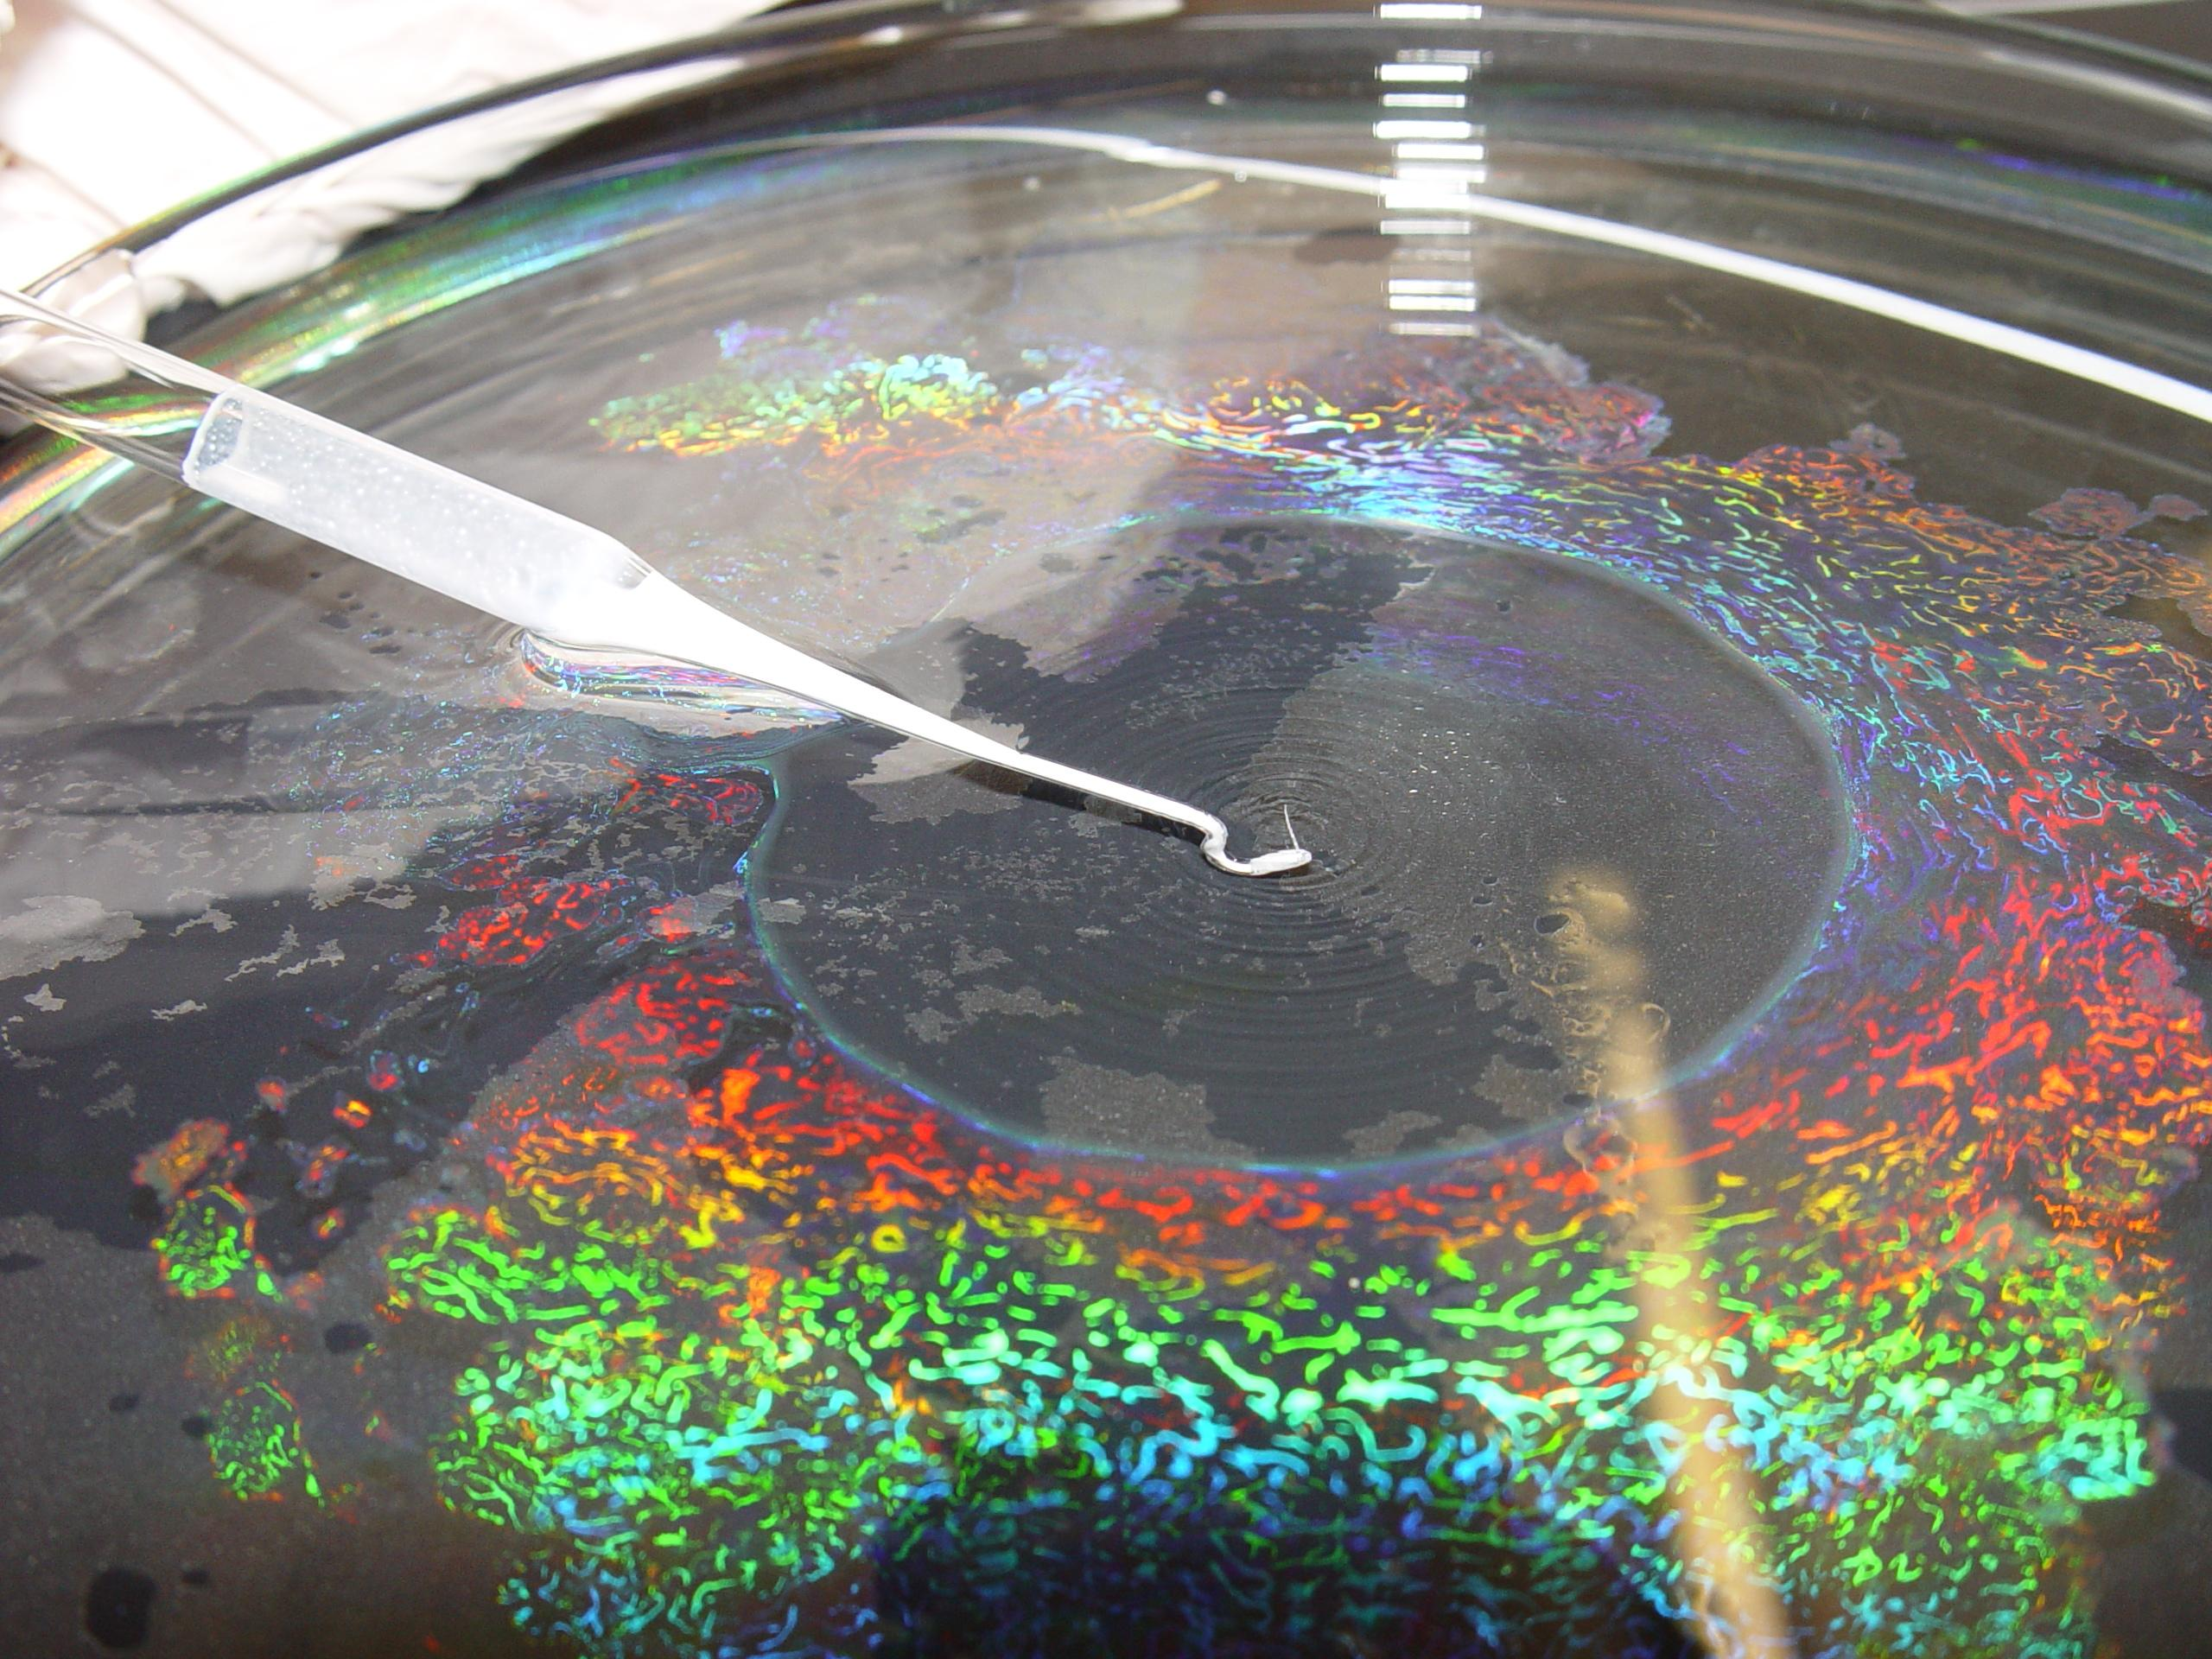
\includegraphics[width=\textwidth]{petrischale.jpg}
\end{subfigure}
\end{figure}